\begin{table*}[]
\caption{server: \textbf{PSC} - \textbf{Detail Slowdown} -
 Inputs: B -
 Nodes: 1 , 4 , 16 , 64 -
 Desc: Detail Report}
\label{det_All_all_B_p3.5}
\begin{center}
\scalebox{0.9}{
\begin{tabular}{|c|c|rrrr|rrrr|rrrr|rrrr|} 
\hline 
\multicolumn{1}{|l|}{\multirow{2}{*}{\textbf{Input: B}}} & \multicolumn{1}{r|}{Nodes :}    & \multicolumn{4}{c|}{1}  & \multicolumn{4}{c|}{4} & \multicolumn{4}{c|}{16}  & \multicolumn{4}{c|}{64} \\ \cline{2-18} 
\multicolumn{1}{|l|}{} & \multicolumn{1}{r|}{Detail Tools:} & \multicolumn{1}{c}{npin} & \multicolumn{1}{c}{dpin} & \multicolumn{1}{c}{ParLOT} & \multicolumn{1}{c|}{wpin} & \multicolumn{1}{c}{npin} & \multicolumn{1}{c}{dpin} & \multicolumn{1}{c}{ParLOT} & \multicolumn{1}{c|}{wpin} & \multicolumn{1}{c}{npin} & \multicolumn{1}{c}{dpin} & \multicolumn{1}{c}{ParLOT} & \multicolumn{1}{c|}{wpin} & \multicolumn{1}{c}{npin} & \multicolumn{1}{c}{dpin} & \multicolumn{1}{c}{ParLOT} & \multicolumn{1}{c|}{wpin} \\
\hline
\multirow{9}{*}{All} &  bt  &  1.79  & \cellcolor{blue!25} 1.74  &  2.01  &   9.85  &  1.65  &   1.80  &   3.95  &  11.66  &   2.82  &   4.91  &   6.55  &  19.22  &  5.53  &  7.54  & \cellcolor{blue!25} 7.38  &  35.77 \\
 &  cg  &  3.41  & \cellcolor{blue!25} 2.76  &  3.03  &   5.50  &  4.47  &   4.54  &   8.96  &  15.72  &   6.74  &  10.29  &  12.53  &  26.52  &  5.35  &  7.62  &  8.72  &  28.50 \\
 &  ep  &  4.85  & \cellcolor{blue!25} 4.46  &  4.63  &  71.39  &  3.06  &   3.27  &   3.52  &  23.90  &  10.03  &  10.18  & \cellcolor{blue!25}  6.47  &  19.03  &  4.96  &  5.46  &  6.58  &  11.81 \\
 &  ft  &  2.40  & \cellcolor{blue!25} 2.31  &  2.43  &   7.40  &  4.09  & \cellcolor{blue!25}  4.08  &   7.67  &  10.68  &   5.63  &   6.23  &  10.40  &  15.70  &  5.97  & \cellcolor{blue!25} 5.42  &  5.88  &  17.76 \\
 &  is  &  7.07  & \cellcolor{blue!25} 6.35  &  6.86  &  21.77  &  5.50  & \cellcolor{blue!25}  5.40  &  10.25  & \cellcolor{blue!25} 10.21  &   7.04  & \cellcolor{blue!25}  4.25  &   5.45  &   8.92  &  8.73  & \cellcolor{blue!25} 6.01  &  8.31  &  19.58 \\
 &  lu  &  1.73  & \cellcolor{blue!25} 1.55  &  1.66  &   2.75  &  2.76  &   5.27  &   5.83  &  14.45  &   4.34  & \cellcolor{blue!25}  2.55  &   4.01  &  26.05  &  6.39  & \cellcolor{blue!25} 4.49  &  7.78  &  83.68 \\
 &  mg  &  8.60  & \cellcolor{blue!25} 8.32  &  9.10  &  11.11  &  5.80  &  10.41  & \cellcolor{blue!25}  6.18  &  10.42  &   5.22  & \cellcolor{blue!25}  5.05  &   6.35  &  14.75  &  7.95  & \cellcolor{blue!25} 5.97  &  6.88  &  21.89 \\
 &  sp  &  1.50  &  1.50  &  1.56  &   3.09  &  3.07  &   5.66  & \cellcolor{blue!25}  3.70  &   8.43  &   5.38  & \cellcolor{blue!25}  3.06  &   4.73  &  17.85  &  5.29  &  6.31  &  9.37  &  57.42 \\ \cline{2-18}
 &  GM  &  3.21  & \cellcolor{blue!25} 2.97  &  3.20  &   9.36  &  3.55  &   4.55  &   5.81  &  12.53  &   5.57  & \cellcolor{blue!25}  5.20  &   6.61  &  17.63  &  6.15  & \cellcolor{blue!25} 6.02  &  7.53  &  28.54 \\
\hline 
\end{tabular} }

\end{center}
\end{table*}

\begin{figure*}[!t]
\centering
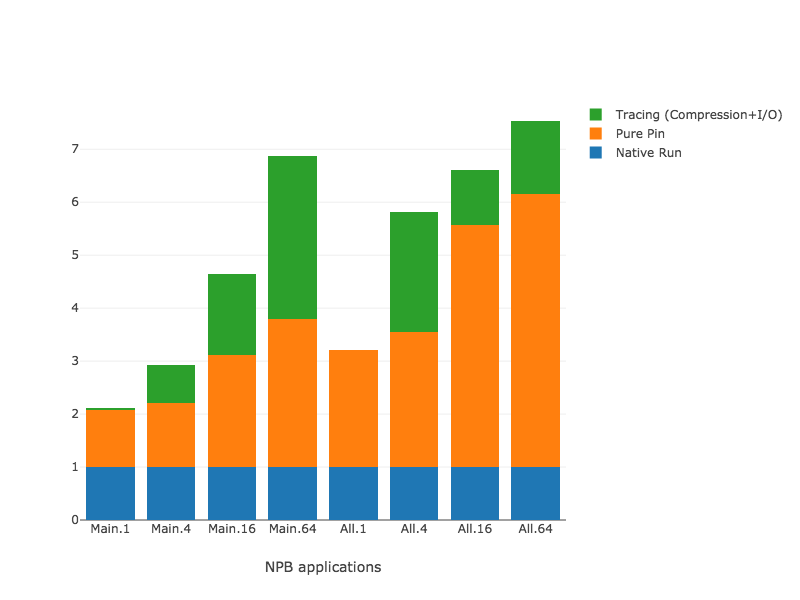
\includegraphics[width=5in]{figs.psc/chartDet_B_wc_byTool_p3_5.png}
\caption{Server: \textbf{PSC} - Input size: \textbf{B}. Each bar is stacked value of slowdowns : $Native Run = 1$ , $Pure Pin = npin - 1$ , $Tracing = ParLOT - npin$. Label of each bar is, (main/all).(1/4/16/64). This graph shows why ParLOT does not scale that well. The overhead that Pin itself is adding to the native run is growing with higher number of cores. The green part of each bar (tracing) is the overhead that our approach is adding. Fig \ref{chartDet_B_woc_byTool_p3_5} shows the effectiveness of our compression approach}
\label{chartDet_B_wc_byTool_p3_5}
\end{figure*}


\begin{figure*}[!t]
\centering
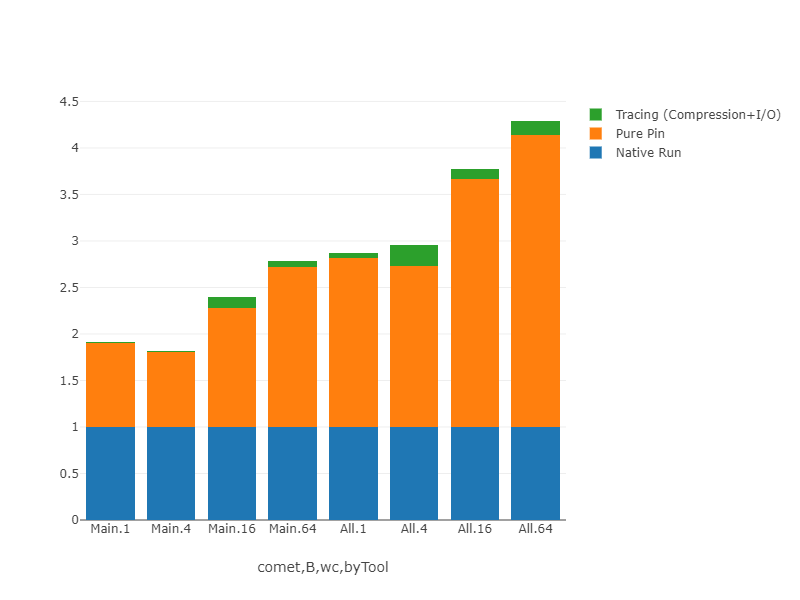
\includegraphics[width=5in]{figs.comet/comet_chartDet_B_wc_byTool_p3_5.png}
\caption{Server: \textbf{Comet} - Input size: \textbf{B}. Similar to fig \ref{chartDet_B_wc_byTool_p3_5}}
\label{chartDet_B_wc_byTool_p3_5}
\end{figure*}

\begin{figure*}[!t]
\centering
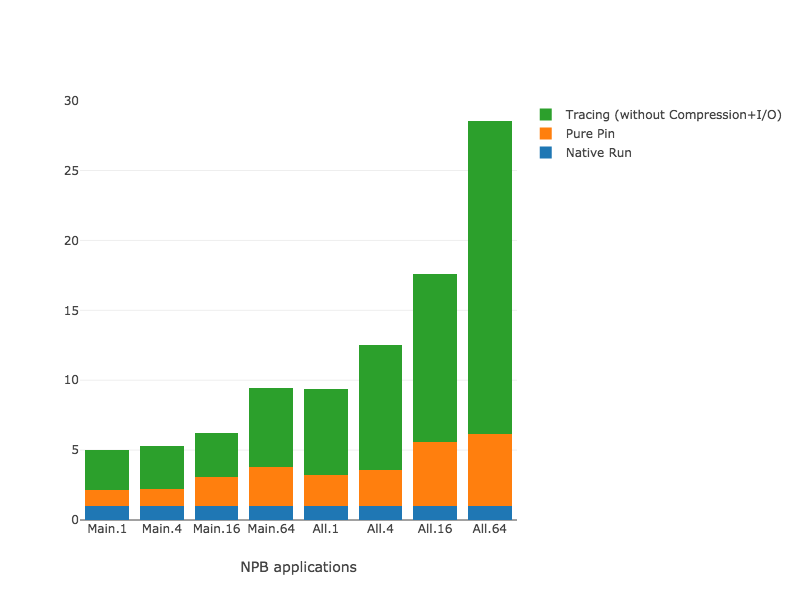
\includegraphics[width=5in]{figs.psc/chartDet_B_woc_byTool_p3_5.png}
\caption{ Server: \textbf{PSC} - Input size: \textbf{B}. Each bar is stacked value of slowdowns : $Native Run = 1$ , $Pure Pin = npin - 1$ , $Tracing (w/o \_compression) = wpin - npin$.
This graph clearly shows how much impact our compression method has on the performance of ParLOT.
}
\label{chartDet_B_woc_byTool_p3_5}
\end{figure*}


\begin{figure*}[!t]
\centering
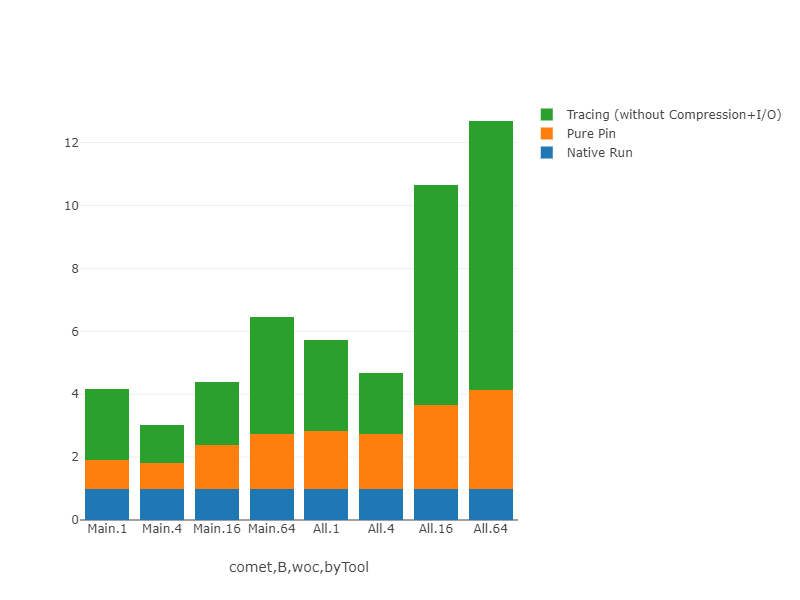
\includegraphics[width=5in]{figs.comet/comet_chartDet_B_woc_byTool_p3_5.png}
\caption{ Server: \textbf{Comet} - Input size: \textbf{B}. Each bar is stacked value of slowdowns : $Native Run = 1$ , $Pure Pin = npin - 1$ , $Tracing (w/o \_compression) = wpin - npin$.
This graph clearly shows how much impact our compression method has on the performance of ParLOT.
}
\label{comet_chartDet_B_woc_byTool_p3_5}
\end{figure*}